\chapter{Data exploration}
Now that the data has been normalized, we thought it natural to explore the data, and see if we could find something. The first thing we thought of was using \textit{clustering}. We thought of using \textit{k-means clustering}, and again we used the function \textit{sklearn}. One can see an example of how we implemented this:

\begin{python}
from sklearn.cluster import KMeans
...
def kmeans_cluster(data, n_clusters):
    kmeans = KMeans(n_clusters=n_clusters)
    kmeans.fit(data)
    y_kmeans = kmeans.predict(data)
    plt.scatter(data[:, 0], data[:, 1], c=y_kmeans, s=50, cmap='viridis')
    centers = kmeans.cluster_centers_
    plt.scatter(centers[:, 0], centers[:, 1], c='black', s=200, alpha=0.5)
...
\end{python}

One can also see an example of the resulting plot from taking the \textit{combined\_2mers} from the folder \textit{processed\_data/combined\_data/with\_background} here:

\begin{figure}[H]
	\centering
	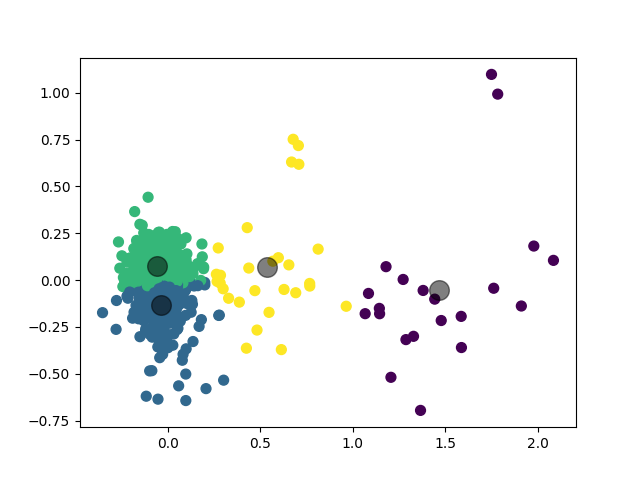
\includegraphics[width=0.7\linewidth]{../../figures/with_background/combined_2mers.png}
	\caption{A k-means clustering of the combined 2-mers file}
	\label{fig:kmeans0}
\end{figure}

Since we have; methylated/unmethylated, cancer/healthy. Which would result in four groupings of the data. We chose to make 4 clusters of the data.

The figure above is for our data normalized with the background, we have also looked into how the clusters look just normalizing each sample individually by looking at the ratios within the sample.

\begin{figure}[H]
	\centering
	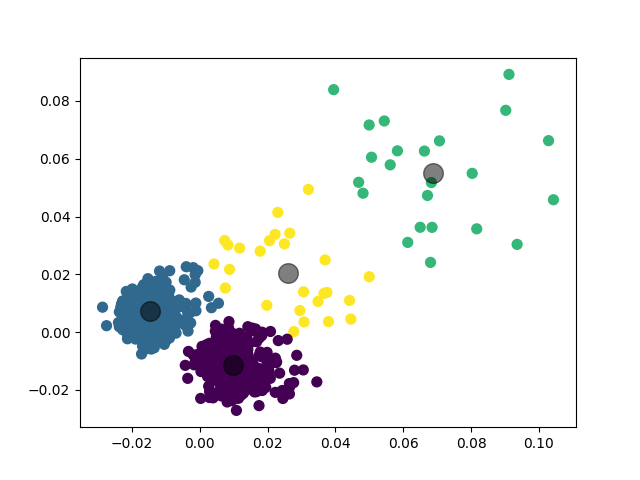
\includegraphics[width=0.7\linewidth]{../../figures/without_background/combined_2mers.png}
	\caption{A k-means clustering of the combined 2-mers file wihtout proper normalization}
	\label{fig:kmeans1}
\end{figure}

As you can see the divide between clusters is somewhat more clear here, however the eventual goal is distinguishing our cases from controls is more difficult using this form of normalization.

\section{Even and Odd}
In order to test our normalization we had the data split into only taking the even/odd lines from each sample, therefore meaning that there should be a noticeable difference between odds and evens despite both being either methylated or unmethylated. To make this process more clear we focused purely on the controls. 

Unlike before where we were primarily interested in just seeing whether these clusters just existed, now we are interested in if we are getting 2 distinct clusters for our 4 groups. 

\begin{figure}[H]
	\centering
	\includegraphics[width=0.7\linewidth]{../../figures/all_healthy/all_healthy.png}
	\caption{A PCA plot of the 4 groups}
	\label{fig:allhealthy0}
\end{figure}

Here we are getting 1 large cluster although we are seeing that we are getting close to having 2 separate clusters. There is however 1 very clear outlier that may be affecting the PCA since one of the 2 components we are plotting may just be the variation caused by this outlier. Therefore we removed it and did the same plot again

\begin{figure}[H]
	\centering
	\includegraphics[width=0.7\linewidth]{../../figures/all_healthy/all_healthy_outlier_removed.png}
	\caption{A PCA plot of the 4 groups with the outlier removed}
	\label{fig:allhealthy1}
\end{figure}

As you can see this made the expected 2 clusters more distinct however there is still a large amount of overlap. We were not able to improve on this using only 2 principal components, although as we will detail later on we were able to clearly distinguish the 2 clusters using more principal components. 
For the sake of clarity we also looked into what this plot would look like without any form of normalization and just looking at the raw data.

\begin{figure}[H]
	\centering
	\includegraphics[width=0.7\linewidth]{../../figures/all_healthy/all_healthy_outlier_removed_raw.png}
	\caption{A PCA plot of the 4 groups with the outlier removed without normalization}
	\label{fig:allhealthy2}
\end{figure}

Much like in our initial exploration we can can see a more clear methylated/unmethylated divide. However, it is becoming more apparent why we need to normalize as there is a large amount of variance in the values of our principal components, making a later distinguishment of controls against cases more difficult 